\documentclass{beamer}
\usetheme{Berlin}
\usecolortheme{beaver}
\usepackage{graphicx}
\usepackage[export]{adjustbox}
\usepackage{tikz}
\usetikzlibrary{arrows}
\usepackage{amsmath}
\usepackage{lmodern}% http://ctan.org/pkg/lm
\usepackage{mathtools}
\usefonttheme{professionalfonts}

\title{Appendix: noise}
\subtitle{}
\author[Riccardo \and Eren]{Riccardo~Miccini\inst{1} \and Eren~Can~\inst{1}}
\institute[DTU]
{
	\inst{1}
	Technical University of Denmark\\
	Digital Communication
}
\date{\today}
\subject{Digital Communication}

\tikzstyle{int}=[draw, fill=blue!20]
\tikzstyle{every node}=[font=\tiny]

\begin{document}
\frame{\titlepage}

% ch A.2
\begin{frame}
	\frametitle{Characterization of noise in systems}
	\begin{itemize}
		\item Noise can be modeled and characterized on a subsystem-basis
		\item Each subsystem can be analyzed separately and optimized for low noise performances
	\end{itemize}
	\begin{figure}
		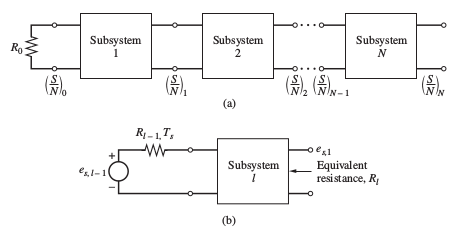
\includegraphics[width=0.8\textwidth]{subsys.png}
	\end{figure}
\end{frame}


% ch A.2.1
\begin{frame}
	\frametitle{Noise Figure of a System}
	\begin{itemize}
		\item Noise figure $F_l$: ratio between SNR at subsystem input and output: $ \left(\frac{S}{N}\right)_l = \frac{1}{F_l} \left(\frac{S}{N}\right)_{l-1} $
		\item Ideally, $ F_l = 1 $ (no additional noise introduced), tipically between 2 and 8 $dB$
		\item Without having to calculate the signal power: $ F_l = 1 + \frac{P_{int,l}}{G_a k T_0 B} $
		\begin{description}
			\item[$P_{int,l}$] Available, internally-generated noise power
			\item[$G_a$] Available power gain
			\item[$k$] Boltzmann's constant
			\item[$T_0$] Standardized temperature, $290 K$
			\item[$B$] Frequency band
		\end{description}
		\item For high gains, $F_l$ approaches 1
	\end{itemize}
\end{frame}


% ch A.2.3
\begin{frame}
	\frametitle{Noise Temperature}
	\begin{itemize}
		\item Power produced by a noisy resistor: $ P_{a,R} = kTB $
		\begin{description}
			\item[$k$] Boltzmann's constant, $ 1.38 \times 10^{-23} J/K $
			\item[$T$] Temperature of the resistor, in Kelvin
			\item[$B$] Frequency band, in Hertz
			\item[] Noise power independent on the resistor value
		\end{description}
		\item Equivalent noise temperature: $ T_n = \frac{P_{n,max}}{kB} $
	\end{itemize}
\end{frame}


\end{document}
